%tout ce qui est dans ce chapitre doit etre succint%
%l'approfondissement se fera dans la seconde partie avec%
%le cas d'étude%

\chapter{Qu'est ce que l'Intelligence Artificielle ?}
L'intelligence Artificelle est un domaine faisant partie 
des sciences cognitives dont l'objectif est de mettre au
point des techniques et technologies permettant aux 
machines de simuler l'intelligence humaine ou animale. 
\newline
Il existe deux type majeur d'intelligence artificielle:
\begin{itemize}
    \item Intelligence artificielle faible, elle reproduit
    un comportement de manière le plus précise possible,
    en s'ameliorant notamment grâce à l'apprentissage 
    mais n'en imite pas le fonctionnement ce qui fait que
    ce type d'IA ne fait qu'imiter l'intelligence.
    % developper pour prendre 1 pages 
    

    \item Intelligence artificelle forte, 

    %developper pour prendre 1 pages 
\end{itemize} 
\begin{figure}[!h]
    \centering
    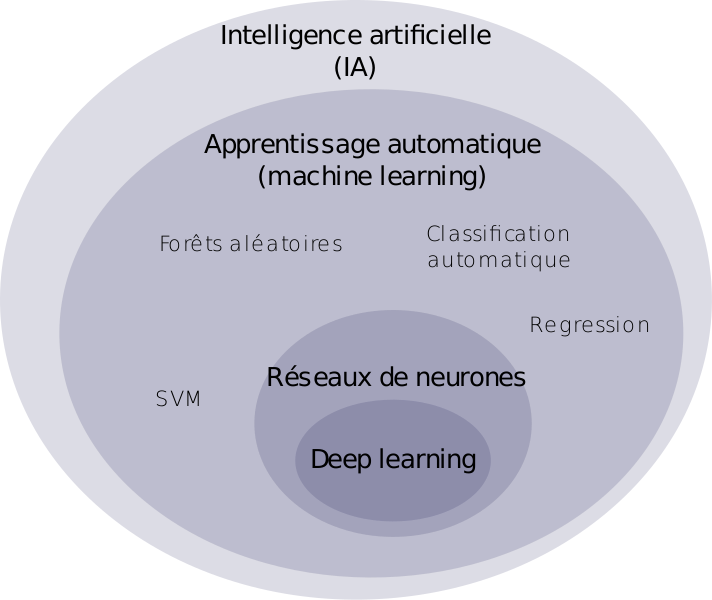
\includegraphics[width=0.8\textwidth]{Images/aitype}
    \caption{Catégories de l'Intelligence Artificielle}
	\label{fig:categorieIA}
\end{figure}

\newpage
\section{Machine Learning}
%trouver des illustration pour facilité la compréhension%
%donner de simple exemple concret% 

\newpage
\section{Deep Learning}
%trouver des illustrations aussi%
%trouver des exemples: Deepmind, watson etc%
Le deep learning est un subset du machine learning, 

\chapter{}